% Some commands used in this file
\newcommand{\package}{\emph}

\chapter{Introduction}
\section{Background}
Managing a large fleet of vehicles requires enormous effort. In order to minimize downtime and offer seamless operation, it is important to monitor the whole fleet on the road. Costs associated with operation, fuel, and maintenance can quickly mount. To ensure that fleet operations are as efficient and cost-friendly as possible, solutions are required to identify and eliminate any unnecessary expenditures. But it is not all about the vehicle itself, there are other factors to be considered. During vehicle operation, the driver can be assisted and warned to ensure safe driving behavior. In general, fleet monitors can be used to improve efficiency, safety, and quality of fleet operations through the use of internet-connected sensors and software.

\section{Scope}
A dedicated device has been developed according to the requirements of our industry partner. A custom \acrshort{pcb} was developed and manufactured. To house the electronics, a water-resistant case was selected and mechanical drawings were created to machine it in the workshop. 

Firmware was written to handle all aspects of operation. An \acrshort{http} server was set up on a Raspberry Pi to receive and log incoming data. Furthermore, software utilities were developed to help the user visualize the collected data and configure the final product. 

The Fleet-Monitor was tested over an extended period with a J1939 simulator to prove its functionality. Documentation, as well as a comprehensive manual, was written for future use.

\newpage
\section{Approach}
Developed by European commercial vehicle manufacturers, the \acrfull{fms} is a common standard for telematics applications. Both driving and diagnostic information can be gathered through this interface. This data is coded to a \acrshort{can} bus, which makes it accessible to third-party devices. For the collection of vehicle data via the \acrshort{fms} interface, a dedicated device was developed.

The Fleet-Monitor is based on an \gls{esp32}-S2 \acrlong{soc} and all of the software is written in C++. Directly connected to the \acrshort{fms} interface, the device collects and filters incoming data, then transmits it over Ethernet or WiFi to the host device. Furthermore, a motion sensor was incorporated to monitor driving performance. 
\bigskip
\begin{figure}[h!]
	\centering
	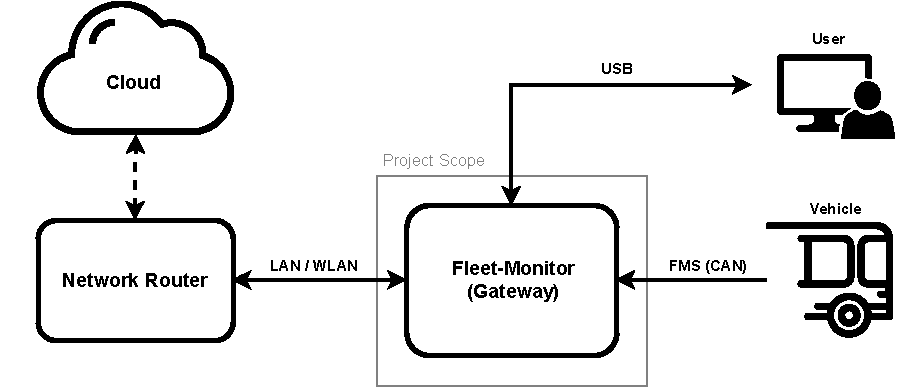
\includegraphics[width=\textwidth]{images/System_Overview}
	\vspace{-0.3cm}
	\caption{System Overview}
	\label{fig:system-overview}
\end{figure}

Utility tools for the generating configuration files, visualizing data, and a \acrshort{http} server were developed. These are needed to support the hardware in its operation. 

\section{Open Source}
From the beginning, it was decided that everything about the project would be released under an open source license. Both of us are huge supporters of open source and believe it will be the future of engineering. Building upon existing libraries and code under open source licenses, allows us to accelerate the design process. Sometimes open source is considered an act of charity, but in our case, the benefits of using it outweigh any closed source processes. All documents and files for this project can be found on our GitHub page. A short description of all the repositories can be found in the Appendix \ref{Data Archive}.
